\documentclass[a4paper, justified]{tufte-handout}

\title{Die Wahrheit der Gewissheit seiner selbst}%\thanks{Inspired by Edward~R. Tufte!}}

%\author[Lennard Wolf]{Lennard Wolf}

\date{ } % without \date command, current date is supplied

%\geometry{showframe} % display margins for debugging page layout

\usepackage{graphicx} % allow embedded images
  \setkeys{Gin}{width=\linewidth,totalheight=\textheight,keepaspectratio}
  \graphicspath{{graphics/}} % set of paths to search for images
\usepackage{amsmath}  % extended mathematics
\usepackage[ngerman]{babel}
\usepackage{booktabs} % book-quality tables
\usepackage{units}    % non-stacked fractions and better unit spacing
\usepackage{multicol} % multiple column layout facilities
\usepackage{lipsum}   % filler text
\usepackage{fancyvrb} % extended verbatim environments
\usepackage{textcomp}
\usepackage{enumitem}
  \fvset{fontsize=\normalsize}% default font size for fancy-verbatim environments

% Standardize command font styles and environments
\newcommand{\doccmd}[1]{\texttt{\textbackslash#1}}% command name -- adds backslash automatically
\newcommand{\docopt}[1]{\ensuremath{\langle}\textrm{\textit{#1}}\ensuremath{\rangle}}% optional command argument
\newcommand{\docarg}[1]{\textrm{\textit{#1}}}% (required) command argument
\newcommand{\docenv}[1]{\textsf{#1}}% environment name
\newcommand{\docpkg}[1]{\texttt{#1}}% package name
\newcommand{\doccls}[1]{\texttt{#1}}% document class name
\newcommand{\docclsopt}[1]{\texttt{#1}}% document class option name
\newenvironment{docspec}{\begin{quote}\noindent}{\end{quote}}% command specification environment

\begin{document}

\maketitle% this prints the handout title, author, and date
\marginnote{Theologische Fakult"at, HU zu Berlin\\Seminar: \\\indent \emph{Hegels Ph"anomenologie des Geistes}\\\noindent Dozent:\\\indent \emph{Dr. D. Karydas}\\\noindent Referent:\\\indent \emph{Lennard Wolf}\\Sommersemester 2017}

\begin{abstract}
\noindent
\emph{"`Was f"ur das Bewu"stsein weiter wird, ist die Erfahrung, was der Geist ist, diese absolute Substanz, welche in der vollkommenen Freiheit und Selbstst"andigkeit ihres Gegensatzes, n"amlich verschiedener f"ur sich seiender Selbstbewu"stsein, die Einheit derselben ist; Ich, das Wir, und Wir, das Ich ist."' (S. 127)}

\end{abstract}

%\printclassoptions

\section{Kontext}\label{sec:context}

Im vorherigen Kapitel endet Hegel damit, dass im Folgenden die Grundlage f"ur das "`Erkennen dessen, was das Bewu"stsein wei"s, indem es sich selbst wei"s"' (S. 119)\footnote{In diesem Thesenpapier entspricht die Seitenangabe der Ausgabe des Meiner Verlags.} geschaffen wird.

\section{Begriff und Gegenstand}\label{sec:context}

\emph{"`Nennen wir Begriff die Bewegung des Wissens, den Gegenstand aber, das Wissen als ruhige Einheit, oder als Ich, so sehen wir, da"s nicht nur f"ur uns, sondern f"ur das Wissen selbst der Gegenstand dem Begriffe entspricht."'} (S. 120)

%Abbildung \ref{fig:begriff} stellt den Begriff als Prozess und den Gegenstand als die ruhige Einheit da, die aber beide, da wir prozesshaft denken, f"ur uns das selbe sind. 

\begin{marginfigure}%
  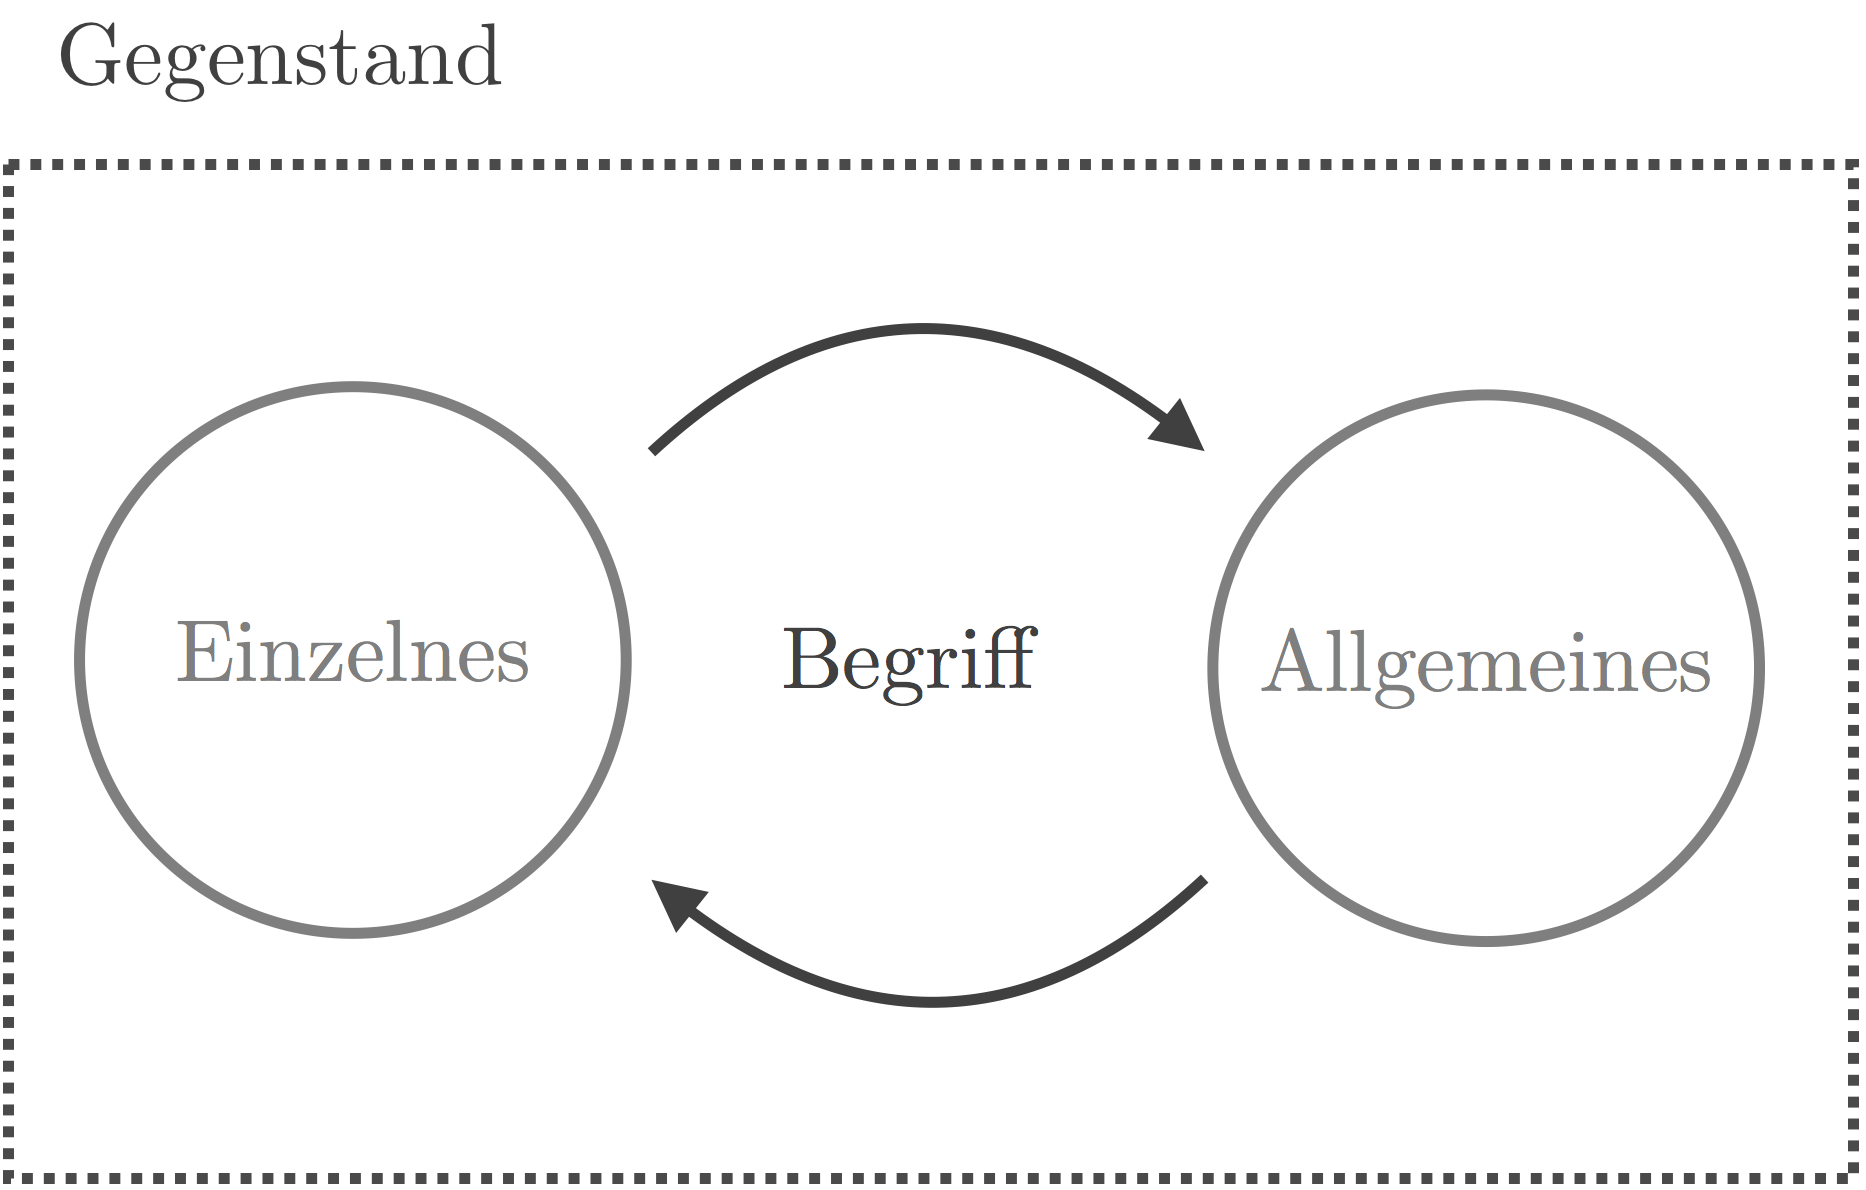
\includegraphics[width=\linewidth]{begriff}
  \caption{Begriff und Gegenstand}
  \label{fig:begriff}
\end{marginfigure}


\section{Unterschiedenes und Ununterschiedenes}\label{sec:leben}

\begin{description}[leftmargin=!,labelwidth=\widthof{\bfseries Neg. d. Neg}]
  \item[Meinen] Die "`fl"ussige Substanz"'\footnote{Dieser abstrakte Begriff wird wohl im weiteren Verlauf durch "`Geist"' ersetzt.} als ununterschiedene Einheit, als "`reine achsendrehende Bewegung"', als "`absolutunruhige Unendlichkeit"' (das \emph{Ansich}).
  \item[Negation] Entzweiung\marginnote{\emph{"`[D]ies Entzweien der unterschiedslosen Fl"ussigkeit ist eben das Setzen der Individualit"at."' (S. 124)}} zu selbst"andigen Gestalten als Bestimmte  (das \emph{Andere f"ur sich}) | Aber: die Gestalten bestehen aus der "`Substanz"' und sind so immer an diese gebunden.
  \item[Neg. d. Neg.] Die "`fl"ussige Substanz"' als ununterschiedene Einheit, die aber der unendliche Unterschied ist.
  \item[Erkenntnis] Das\marginnote{\emph{"`Dieser ganze Kreislauf macht das Leben aus, [...] das sich entwickelnde, und seine Entwicklung aufl"osende und in dieser Bewegung sich einfach erhaltende Ganze."'} (S. 125)} Ganze und das Individuelle bedingen einander. Das Leben ist f"ur das Selbstbewusstsein die Einheit, oder Gattung.
\end{description}


\section{Selbstbewusstsein}\label{sec:page-layout}

Da\marginnote{\emph{"`Nunmehr aber ist dies entstanden, was in diesen fr"uhern Verh"altnissen nicht zustande kam, n"amlich eine Gewi"sheit, welche ihrer Wahrheit gleich ist, denn die Gewi"sheit ist sich selbst ihr Gegenstand, und das Bewu"stsein ist sich selbst das Wahre."'} (S. 120)} in den "Uberlegungen dieses Abschnitts das Bewusstsein sich selbst thematisiert, f"allt zu allererst auf, dass es gleichzeitig Bewusstsein und Gegenstand zugleich ist. So ist der Gegenstand dem Bewusstsein hier als Gewissheit aber nicht von der Wahrheit getrennt.

\begin{description}[leftmargin=!,labelwidth=\widthof{\bfseries Neg. d. Neg}]
  \item[Meinen] Selbstbewusstsein als unmittelbares Bewusstsein vom \emph{ununterschiedenen Ich}.
  \item[Negation] Selbstbewusstsein\marginnote{\emph{"`Indem ein Selbstbewu"stsein der Gegenstand ist, ist er ebensowohl Ich, wie Gegenstand."'} (S. 127)} als Bewusstsein von sich selbst als \emph{Anderem} Sein. | Aber: der Unterschied \emph{ist} nicht, "`Ich bin Ich"' ist bewegungslose Tautologie: hier ist keine sinnliche Wahrnehmung, hier ist kein Proze"s.
  \item[Neg. d. Neg.] Selbstbewusstsein\marginnote{\emph{"`Das Selbstbewu"stsein stellt sich hierin als die Bewegung dar, worin dieser Gegensatz aufgehoben, und ihm die Gleichheit seiner selbst mit sich wird."'} (S. 122)} als unmittelbares Bewusstsein vom ununterschiedenen Ich, das eine unerf"ullte Begierde danach hat, wahrgenommen zu werden.
  \item[Erkenntnis] Befriedigung\marginnote{\emph{"`Das Selbstbewu"stsein erreicht seine Befriedigung nur in einem andern Selbstbewu"stsein."'} (S. 126)} der Einheit seiner Selbst als unmittelbares Bewusstsein in einem Anderssein muss durch ein anderes Bewusstsein erreicht werden.
\end{description}

%\subsection{Auswahl}
%
%\begin{figure*}[h]
%  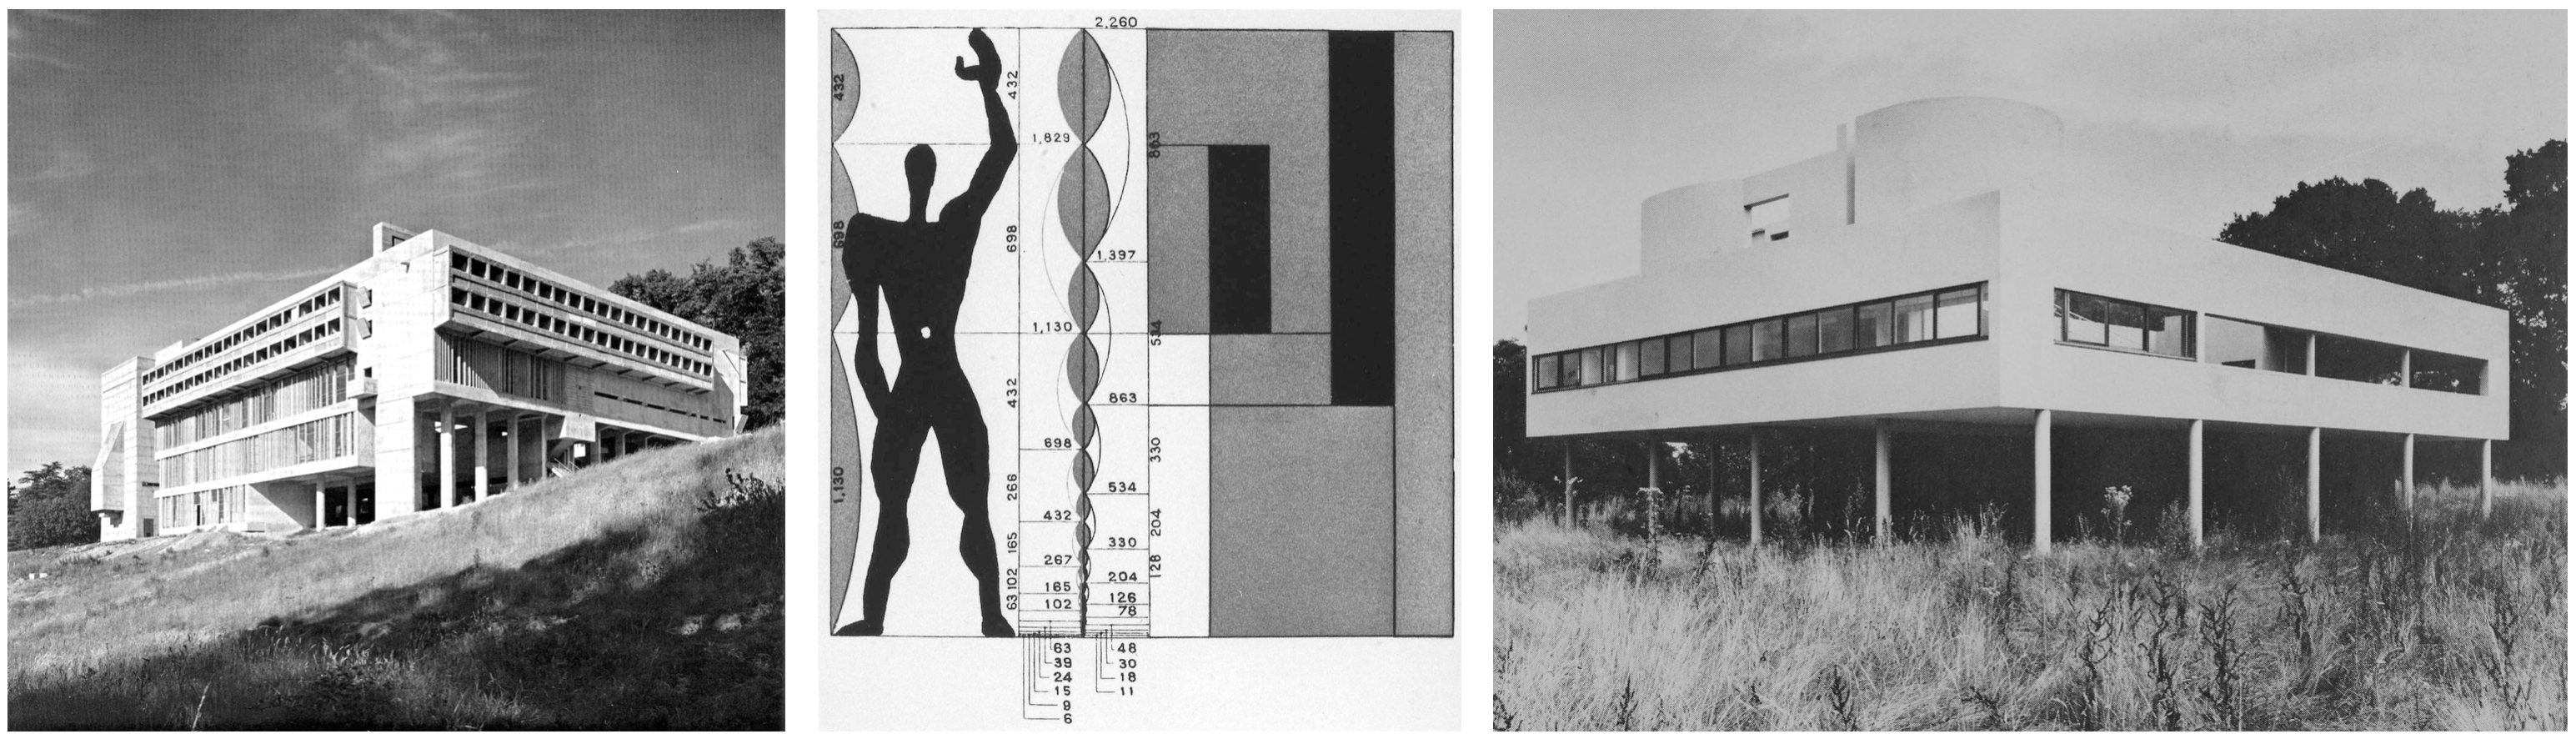
\includegraphics[width=\linewidth]{slideshow}%
%  \caption{La Tourette, der Modulor, Villa Savoye}%
%  \label{fig:fullfig}%
%\end{figure*}

%\begin{fullwidth}
%\small\itshape\lipsum[1]
%\end{fullwidth}


%\footnote{This is a sidenote that was entered
%using the \texttt{\textbackslash footnote} command.}  
%
%\marginnote{This is a
%margin note.  Notice that there isn't a number preceding the note, and
%there is no number in the main text where this note was written.}
%
%\sidenote{The first paragraph of this document includes a citation.}



%\section{Literatur}\label{sec:lit}
%
%\begin{fullwidth}
%
%\noindent von Vegesack, Alexander (Hrsg.): \emph{Le Corbusier - The Art of Architecture}, Weil am Rhein 2007.\\
%
%\noindent Le Corbusier: \emph{New World of Space}, New York 1948.\\
%
%\noindent Le Corbusier: \emph{Vers une architecture}, Paris 1923.\\
%
%\noindent Dalrymple, Theodore: \emph{"`Der totalit"are Architekt. Le Corbusiers unheilvoller Einfluss dauert an"'}, in: Merkur, Heft 04, Stuttgart 2010.\\
%
%\noindent Gargiani, Roberto/ Rosellini, Anna: \emph{Le Corbusier. B\'eton Brut und der Unbeschreibliche Raum (1940 -- 1965): Oberfl"achenmaterialien und die Psychophysiologie des Sehens}, M"unchen 2014.\\

%\end{fullwidth}
%\nocite{*}
%\bibliography{corbusier}
%\bibliographystyle{plainnat}



\end{document}
